% scan-paragraphs — paragraphs.pdf as a flatbed scanner returns it: one page image and no text.
%
% scan-paragraphs.jpg is paragraphs.pdf rendered at 200 dpi and passed through degrade.go: grey, a
% 0.6 degree skew, a paper tone, sensor noise, and JPEG at quality 60. pdfTeX embeds
% the JPEG as it is, under /DCTDecode, which is what scanners write. Nothing on the
% page is text, so every word the converter returns came from reading pixels, and
% the gold file is paragraphs.gold.md's, because the document is the same one.
\documentclass{article}
\usepackage{graphicx}
\usepackage[paperwidth=8.2700in,paperheight=11.6950in,margin=0in]{geometry}
\pagestyle{empty}
\setlength{\topskip}{0pt}
\setlength{\parindent}{0pt}
\begin{document}
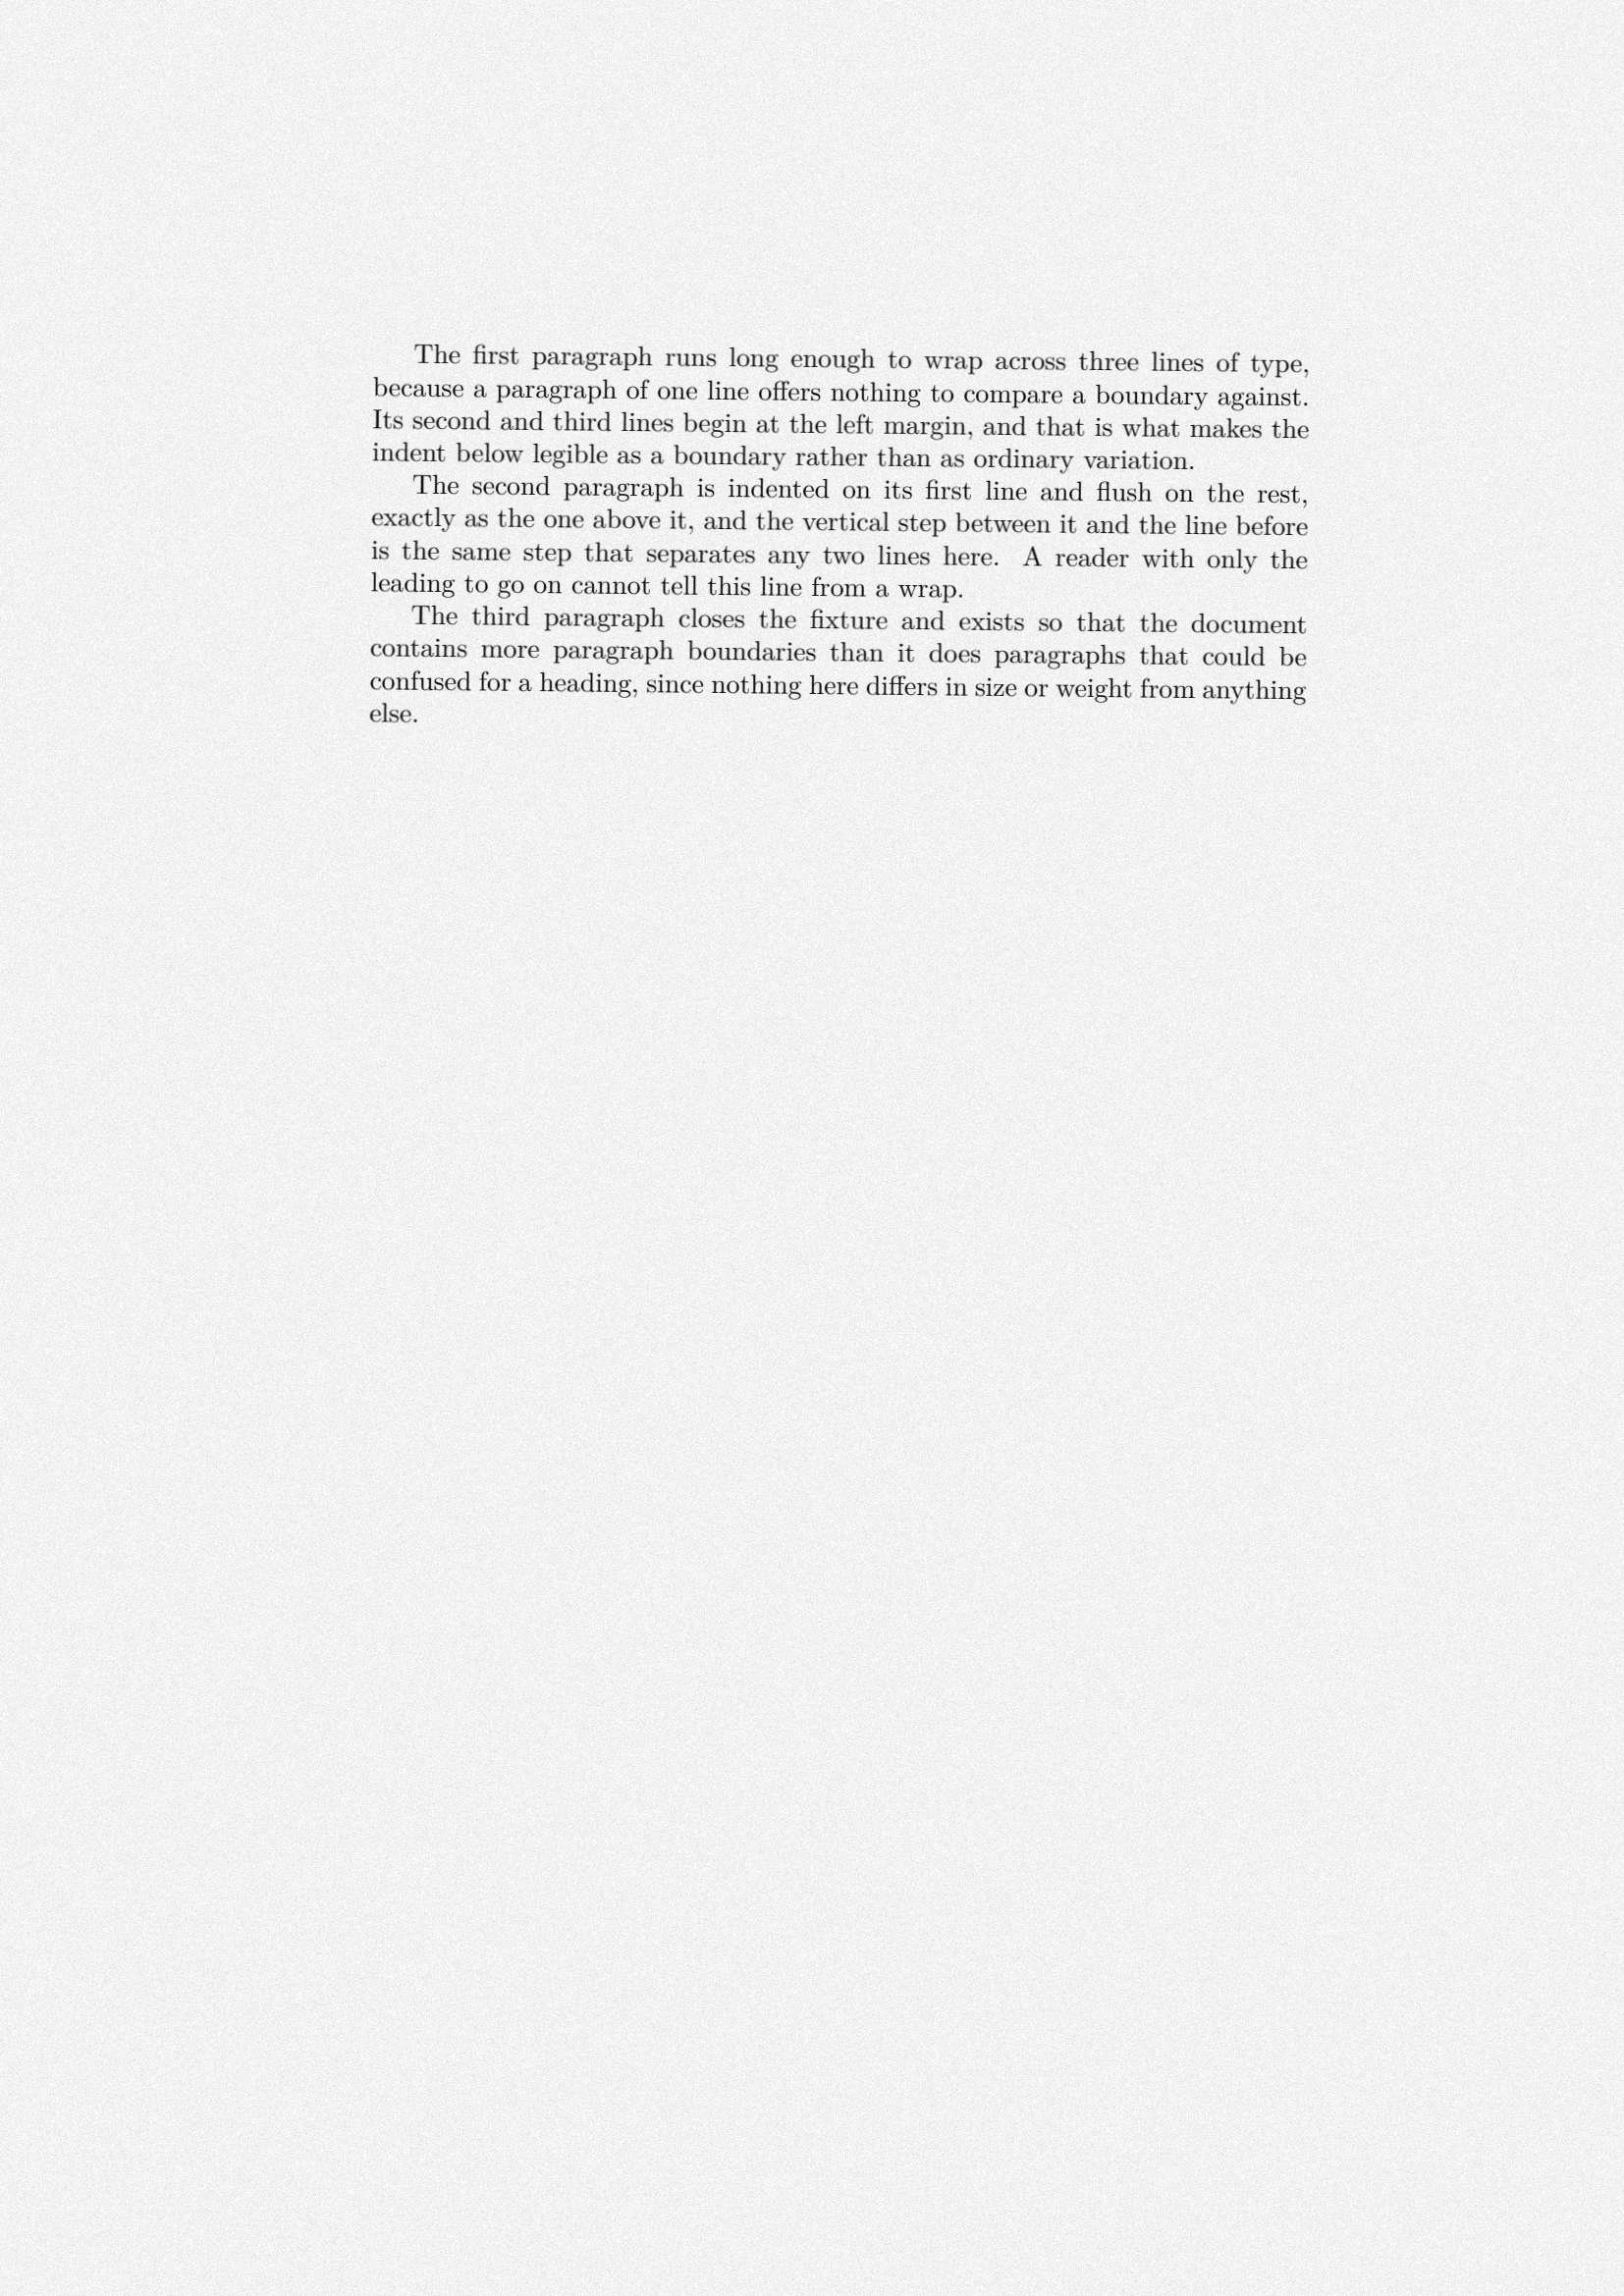
\includegraphics[width=\paperwidth,height=\dimexpr\paperheight-1pt\relax]{scan-paragraphs.jpg}
\end{document}
